\documentclass{beamer}
\usetheme{Boadilla}
\usecolortheme{sidebartab}

\usepackage{hyperref}
\usepackage{showexpl} 
\usepackage{graphicx}
\usepackage{color}
\usepackage{siunitx}
\usepackage[version=3]{mhchem}
\usepackage{chemfig}
\usepackage{changes}
\usepackage[many]{tcolorbox}
\usepackage{natbib}
\bibliographystyle{unsrtnat}
\setcitestyle{square,numbers}

\beamertemplatenavigationsymbolsempty
\setbeamertemplate{footline}{}
\setbeamertemplate{bibliography item}{\insertbiblabel}

\lstloadlanguages{[LaTeX]Tex} 
\lstset{% 
     basicstyle=\ttfamily\large, 
     commentstyle=\itshape\ttfamily, 
     showspaces=false, 
     showstringspaces=false, 
     breaklines=true, 
     breakautoindent=false, 
     captionpos=t,
     explpreset={numbers=none},
     pos=b
} 

\title{Sharing and Archiving Research Data}
\author{Markus Stocker}
\date{September 12, 2017}

\begin{document}

\maketitle

\begin{frame}
  \frametitle{Outline}
  
  \begin{itemize}
  \item Open Data imperative
  \item How to share data
  \item Data repositories
  \item Credit for publishing data
  \end{itemize}
\end{frame}

\begin{frame}
  \frametitle{Open Data}
  
  \begin{itemize}
  \item Research data are assets
  \item Increasingly recognized and valued research output	
  \item Valuable to others, in research as well as industry
  \item Critical for reproducibility
  \item Mandates to open access publicly funded data
  \item Anyone free to use, reuse, and redistribute
  \item Possibly subject to attribution
  \end{itemize}
\end{frame}

\begin{frame}
  \frametitle{Data Identification}
  
  \begin{itemize}
  \item Persistent identification of data is important
  \item Idea is similar to identification of articles
  \item Provides an unambiguous reference to data
  \item Used to link or refer to data, e.g. in text
  \item Data are increasingly identified by DOI 
  \begin{itemize}
  \item e.g. 10.1594/PANGAEA.787617
  \end{itemize}
  \item DataCite is the global provider of DOIs for research data
  \end{itemize}
\end{frame}

\begin{frame}
  \frametitle{Data Citation}
  
  \begin{itemize}
  \item Always cite data used in research
  \item Citing data is often very easy
  \item Data repositories support citation export
  \end{itemize}
\end{frame}

{
	\usebackgroundtemplate{ %
		\begin{tikzpicture}[remember picture, overlay]%
		\node at (current page.center) {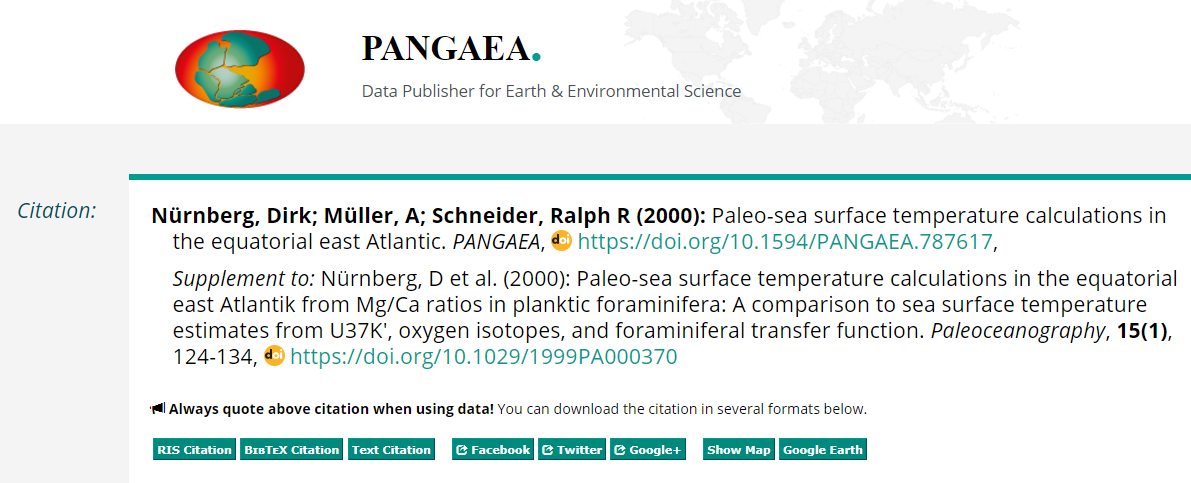
\includegraphics[width=\paperwidth]{graphics/pangaea-datacitation.png}};%
		\end{tikzpicture}%
	}%
	\setbeamertemplate{navigation symbols}{}
	\begin{frame}[plain]
	\end{frame}
}

% https://www.force11.org/group/fairgroup/fairprinciples
\begin{frame}
  \frametitle{FAIR Principles}
  
  \begin{itemize}
  \item Findable
  \begin{itemize}
  \item Persistently identified, described, indexed
  \end{itemize}
  \item Accessible
  \begin{itemize}
  \item Retrievable by identifier, open protocol, accessible metadata
  \end{itemize}
  \item Interoperable
  \begin{itemize}
  \item Represented using formal, accessible, shared FAIR vocabulary
  \end{itemize}
  \item Re-usable
  \begin{itemize}
  \item Meet community standards, associated with provenance, usage license
  \end{itemize}
  \end{itemize}
\end{frame}


\begin{frame}
  \frametitle{Take aways}
  
\end{frame}

\end{document}
